\chapter*{Implementace}
\par V rámci této úlohy bylo ve frameworku QT vytvořené uživatelské prostředí pro načítání dvou liniových prvků. Jeden z prvků představuje objekt, který se má být zgeneralizovat vůči druhému liniovému prvku, představující bariéru.

\section*{Vstupní data}
\par K aplikaci jsou přidaná zkušební data, na kterých lze aplikaci otestovat. Testovací data představují dva soubory typu .csv. V jednom případě se jedná o silniční liniový prvek a v druhém případě o vodní tok. Data se nachází ve složce \verb|/input_files| pod názvy \verb|silnice.csv| a \verb|vodni_tok.csv|. Jejich grafické znázornění je vidět na Obrázku 2.

\begin{figure}[H]
\centering
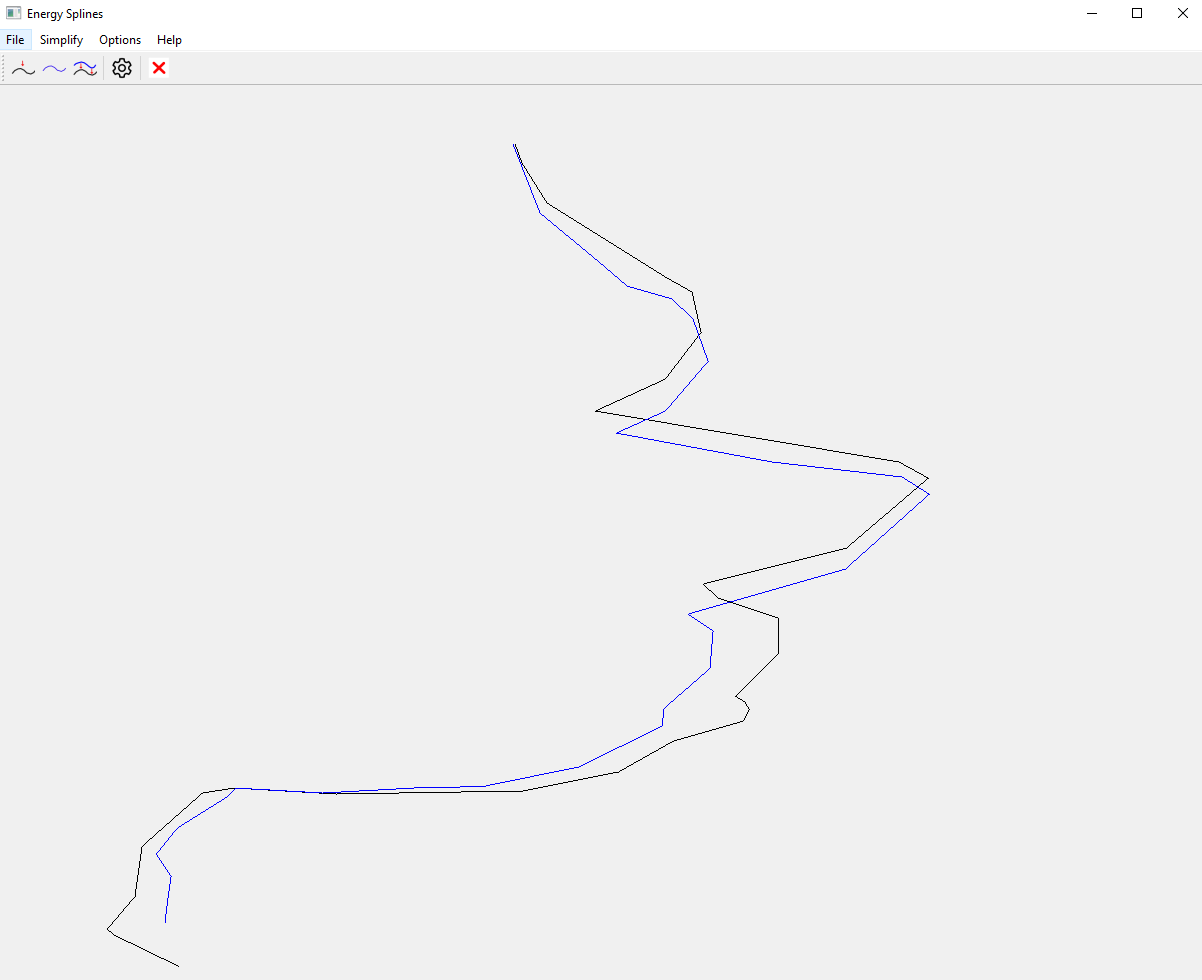
\includegraphics[width=14cm]{data.png}
    \caption{Načtení liniových prvků silnice (černě) a vodního toku (modře) (vlastní zpracování).}
\end{figure}

\section*{Aplikace}
\par Grafické uživatelské prostředí bylo navrhnuto a vygenerováno v rozhraní \verb|Qt Creator 9.0.1|. Samotné výpočetní a doprovodné algoritmy včetně vykreslování dat byly realizovány pomocí programovacího jazyka \verb|Python 3.11|. Obrázek 3 pak názorně ilustruje možnosti grafického prostředí a funkčnost celé aplikace.

\begin{figure}[h]
\centering
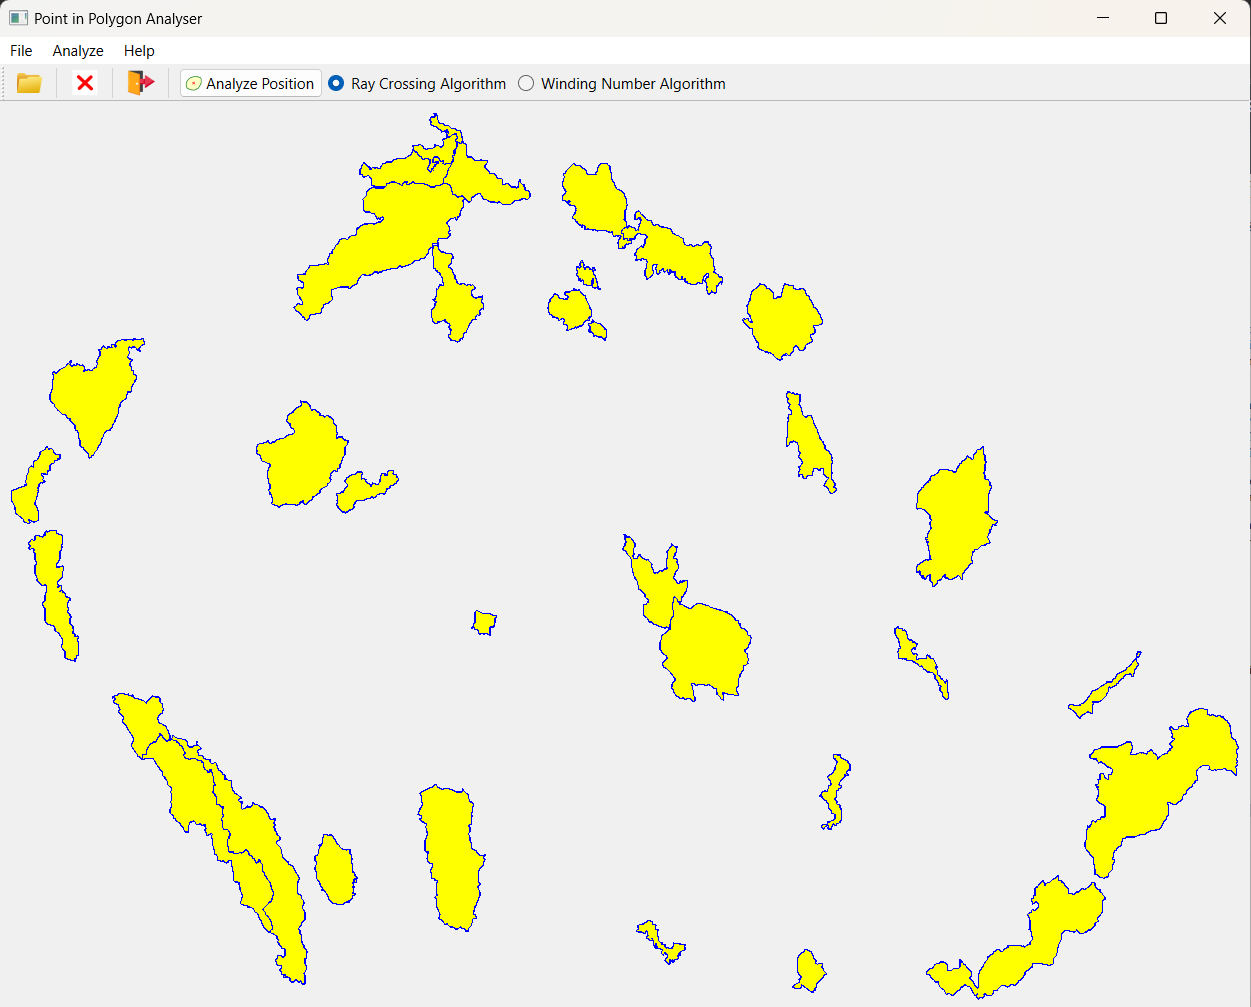
\includegraphics[width=15cm]{showcase.png}
    \caption{Ukázka grafického okna aplikace s popisem funkcí (vlastní zpracování).}
\end{figure}

\par Uživatel si může skrze aplikaci nahrát vstupní data (bariéru a odsunující linii) v podobě .csv souboru. Pomocí tlačítka nebo ikony nastavení (options/settings) je možné upravit parametry pro odsun dle vlastní potřeby. Tyto parametry jsou výchoze nastaveny tak, jak je vidět na Obrázku 3. Vizualizovaná data i grafické výsledky odsunuté křivky je možné smazat pomocí červeného křížku. 

\section*{Třídy a metody}
\par Pro zdárné spuštění aplikace je potřeba následující tři skripty \verb|mainform.py|, \verb|algorithms.py| a \verb|draw.py|, které obsahují třídy \verb|Ui_MainWindow|, \verb|Algorithms| a \verb|Draw|, ve kterých jsou níže popsány jejich jednotlivé algoritmy včetně jejich funkčnosti. 

\par {\large\textbf{Třída Ui\_MainWindow} }

\par Třída Ui\_MainWindow ze souboru \verb|mainform.py| zabezpečuje inicializaci okna aplikace, vrchní lišty, panelu nástrojů, ikon a tlačítek. Zároveň propojuje jednotlivé interaktivní položky okna s metodami, které vykonají specifické akce. Týkají se především otevření souboru, spouštění konkrétních algoritmů apod. Část této třídy byla vygenerována v prostředí \verb|Qt Creator 9.0.1| (metody \verb|setupUi()| a \verb|translateUi()|). Níže jsou vyjmenovány nově implementované metody:

\par 
\begin{itemize}
    \item \verb|__init__()|
        \subitem{Inicializuje výchozí parametry pro výpočet energetického splinu.}
    \item \verb|set SplineSettings()|
        \subitem{Nastavuje vstupní parametry energetického splinu .}
    \item \verb|setSplineDefaultSettings()|
        \subitem{Nastavuje výchozí parametry splinu}
    \item \verb|splineInvalidInput()|
        \subitem{Upozorní na nevalidní vstupní parametry splinu.}
    \item \verb|displaceClick()|
        \subitem{Provede výpočet energetického splinu, respektive odsune potřebný liniový prvek vůči zadané bariéře.}
    \item \verb|loadLineClick()|
        \subitem{Načítá vstupní soubor pro liniový prvek, který se bude generalizovat.}
    \item \verb|loadBarrierClick()|
        \subitem{Načítá vstupní soubor pro liniový prvek, který představuje bariéru.}
    \item \verb|clearClick()|
        \subitem{Vymaže veškeré grafické výsledky.}
    \item \verb|openFile()|
        \subitem{Otevře \verb|CSV| soubor a načte ho do proměnné.}
    \item \verb|processFile()|
        \subitem{Zabezpečuje otevření souboru. Samotný soubor načte do proměnné pomocí metody \verb|openFile()| a následně zavolá metodu \verb|clearCanvas()| pro vyprázdnění okna. Pokud je vstupní \verb|CSV| nečitelný, uživatele na to upozorní vyskakovacím oknem.}
    \item \verb|aboutClick()|
        \subitem{Otevře se Github repozitář s řešeným úkolem, informacemi a dokumentací k této úloze.}
    \item \verb|exitClick()|
        \subitem{Ukončí chod aplikace.}
\end{itemize}

\bigbreak

\par {\large\textbf{Třída Algorithms} }
\par V této třídě jsou obsaženy algoritmy pro výpočet energetického splinu a odsunutí zadaného liniového prvku vůči nějaké bariéře. Třída obsahuje následující metody:

\begin{itemize}
    \item \verb|getEuclidDistance(self, x1, y1, x2, y2)|
        \subitem{Vypočte euklidovskou vzdálenost mezi dvěma body.}
    \item \verb|getPointLineDistance(self, xa, ya, x1, y1, x2, y2)|
        \subitem{Vypočte vzdálenost mezi bodem a linií.}
    \item \verb|getPointLineSegmentDistance(self, xa, ya, x1, y1, x2, y2)|
        \subitem{Vrátí vzdálenost mezi bodem a liniovým segmentem}
    \item \verb|getNearestLineSegmentPoint(self, xa: float, ya: float, X: matrix, Y: matrix)|
        \subitem{Vrátí průsečík (bod) na bariéře. Jedná se o kolmý průmět bodu $p$ na bariéru.}
    \item \verb|createA(self, alpha, beta, gamma, h, m)|
        \subitem{Vytvoří matici A pro účel výpočtu odsunutí liniového prvku.}
    \item \verb|getEx(self, xi, yi, xn, yn, d, dmin)|
        \subitem{Vrátí parciální derivaci pro vnější energii podle x.}
    \item \verb|getEy(self, xi, yi, xn, yn, d, dmin)|
        \subitem{Vrátí parciální derivaci pro vnější energii podle y.}
    \item \verb|minEnergySpline()|
        \subitem{Vytvoří novou odsunutou linii.}
\end{itemize}
\bigbreak

\par {\large\textbf{Třída Draw} }
\par Třída Draw ze souboru \verb|draw.py| slouží pro inicializaci proměnných nesoucí prostorovou informaci, načítání a vykreslování geoprostorové informace. Tato třída má 3 \verb|list| atributů, 4 \verb|int| atributy a 3 \verb|bool| atributy pro manipulaci se vstupními daty.

\par Třída Draw pak obsahuje následující metody:
\begin{itemize}
    \item \verb|paintEvent(self)|
        \subitem{Zodpovídá za veškeré grafické vykreslování na plátno (Canvas).}
    \item \verb|getL(self)|
        \subitem{Vrací liniový prvek, který se bude generalizovat.}
    \item \verb|getB(self)|
        \subitem{Vrací liniový prvek bariéry.}
    \item \verb|setLD(self, LD_)|
        \subitem{Nastaví vytvořenou odsunutou linii.}
    \item \verb|setSource(self, status)|
        \subitem{Přepíná mezi vstupní linií a bariérou. Nese informaci, zda se aktuálně zpracovává generalizovaná linie, nebo bariéra.}
    \item \verb|clearAll(self)|
        \subitem{Smaže všechny objekty na plátně (Canvas).}
    \item \verb|loadData(data)|
        \subitem{Prochází vstupní \verb|CSV| soubor a načte geoprostorovou informaci.}
    \item \verb|findBoundingPoints(p,, xmin, ymin, xmax, ymax)|
        \subitem{Nalezne minimální a maximální souřadnice pro vykreslování vstupních dat.}
    \item \verb|resizeContent(xmin, ymin, xmax, ymax)|
        \subitem{Roztáhne vstupní data na plátno podle velikosti okna aplikace.}
\end{itemize}